\documentclass{beamer}

\usepackage{amsmath}
%\usepackage{color}
\usepackage{tikz}
%\usepackage{graphicx}
%\usepackage{concmath}
\usepackage{pifont}
%\usepackage{setspace}
%\usepackage{enumitem}
%\usepackage{verbatim} 
%\usepackage{multirow}
\usetikzlibrary{arrows,positioning,matrix,shapes,chains,calc}

\usepackage{caption}
\captionsetup{labelformat=empty,labelsep=none}

\usetheme{default}
\usefonttheme{serif}
\usefonttheme{professionalfonts}
\beamertemplatenavigationsymbolsempty
\setbeamertemplate{blocks}[rounded][shadow=true]

\definecolor{Red}{rgb}{0.855,0.0,0.039}
\definecolor{orangered}{rgb}{1,0.10,0}
\definecolor{Blue}{rgb}{0.0,0.235,0.561}
\definecolor{DarkBlue}{rgb}{0.0,0.235,0.561}
\definecolor{Grey}{rgb}{0.255,0.259,0.224}
\definecolor{LBlue}{cmyk}{0.1,0.05,0,0}
\definecolor{LGreen}{cmyk}{0.1,0,0.1,0}
\definecolor{LRed}{cmyk}{0,0.1,0,0}
\definecolor{DarkGreen}{rgb}{0,0.4,0}
\definecolor{DarkTurquiose}{rgb}{0.382,0.307,1}
 
\graphicspath{{Images/}}

%--------------------------------------
% Theorem definitions
%--------------------------------------
\theoremstyle{definition}
\newtheorem{thm}[theorem]{Theorem}
\newtheorem{conjecture}[theorem]{Conjecture}
\newtheorem{cor}[theorem]{Corollary}
\newtheorem{prop}[theorem]{Proposition}
\newtheorem{quest}{Question}
\newtheorem{defn}{Definition}
\newtheorem{mthm}{Main Theorem}
  
\newcommand{\putbox}[1]{\begin{equation*}\addtolength{\fboxsep}{5pt}\boxed{\begin{gathered}#1\end{gathered}} \end{equation*}}
\newcommand{\mS}{\mathcal{S}}
\newcommand{\mA}{\mathcal{A}}
\newcommand{\mB}{\mathcal{B}}
\newcommand{\mC}{\mathcal{C}}
\newcommand{\mD}{\mathcal{D}}
\newcommand{\mE}{\mathcal{E}}
\newcommand{\bi}{\mathbf{i}}
\newcommand{\bz}{\mathbf{z}}
\newcommand{\by}{\mathbf{y}}
\newcommand{\oz}{\overline{z}}
\newcommand{\oy}{\overline{y}}
\newcommand{\ox}{\overline{x}}
\newcommand{\bo}{\mathbf{1}}
\newcommand{\ok}{\ensuremath{\overline{k}}}
\newcommand{\sgn}{\text{sgn}}
\newcommand{\mV}{\mathcal{V}}
\newcommand{\bp}{\mbox{\boldmath$\rho$}}


\titlegraphic{
\includegraphics[scale=0.18]{title.jpg}}


\title{Password Authenticated Key Exchange:\\ From Two Party Methods to Group Schemes \vspace{-0.2in}}
\author{Stephen Melczer, Taras Mychaskiw, and Yi Zhang}
\date{}

\begin{document}
\frame{\titlepage}



%%%%%%%%%%%%%%%%%%%%%%%%%%%%%%%%%%%
% Introduction
%%%%%%%%%%%%%%%%%%%%%%%%%%%%%%%%%%%

\frame{  
  \frametitle{Introduction}
  \begin{enumerate}
  \item Classical Two Party PAKEs
  		\begin{enumerate}
  		\item Background and Security Properties
  		\item J-PAKE
  		\item Dragonfly
  		\item PAK/PPK
  		\end{enumerate}
  \item[]
  \item Extension to Group Setting (GPAKEs)
  		\begin{enumerate}
  		\item Fairy-Ring Dance
  		\item Examples of GPAKEs
  		\end{enumerate}
    \item[]
  \item Timings
    \item[]
  \item Conclusion
  \end{enumerate}
}

%%%%%%%%%%%%%%%%%%%%%%%%%%%%%%%%%%%
% Two Party PAKEs
%%%%%%%%%%%%%%%%%%%%%%%%%%%%%%%%%%%

\frame{
  \frametitle{\vspace{1.1in} \begin{center} PART 1 \\ Classical Two Party PAKEs \end{center}}
}


\frame{  
  \frametitle{Password Authenticated Key Exchange (PAKE)}
  PAKEs allow two parties sharing a \emph{short/weak} password to establish a shared key
  \vspace{0.5in}

  Cannot broadcast password directly -- would need to be protected (expensive)
  \vspace{0.5in}

  Instead, modern PAKEs use \emph{zero-knowledge proof} and/or \emph{hash} of password in protocol
}

\frame{  
  \frametitle{First Protocol: EKE (Bellovin and Merrit 1992)}
  Pick prim. root $\alpha \in \mathbb{Z}_p$
  \vspace{0.4in}

  \scalebox{0.7}{
    \begin{tikzpicture}
        \matrix (m)[matrix of nodes, column sep=2cm, row sep=8mm, nodes={draw=none, anchor=center, text depth=0pt},ampersand replacement=\&]{
            Alice                                       \&                   \& Bob                                       \\
            randomly choose $x_a \in \mathbb{Z}_p^*$    \& $[\alpha^{x_a}]_s$\&                                           \\
                                                        \& $[\alpha^{x_b}]_s$\& randomly choose $x_b \in \mathbb{Z}_p^*$  \\
        };

        % draw the nodes - these are 1-based indicies on the matrix called `m`, ie to draw in (x,y), reference it as `m-x-y`
        \draw[shorten <=-1.5cm,shorten >=-1.5cm] (m-1-1.south east)--(m-1-1.south west);    % underline "Alice"
        \draw[shorten <=-1.5cm,shorten >=-1.5cm] (m-1-3.south east)--(m-1-3.south west);    % underline "Bob"
        \draw[shorten <=-1cm,shorten >=-1cm,-latex] (m-2-2.south west)--(m-2-2.south east); % arrow below sending alpha^x_a
        \draw[shorten <=-1cm,shorten >=-1cm,-latex] (m-3-2.south east)--(m-3-2.south west); % arrow below sending alpha^x_b
    \end{tikzpicture}}
    \vspace{0.2in}

	Alice and Bob share $K = \alpha^{x_a \cdot x_b}$.    
    \vspace{0.6in}

\pause
Uses password directly $\implies$ many insecurities found
\vspace{0.2in}

\pause
Ex: Decypher $[\alpha^{x_a}]_{s'}$ -- rule out $s'$ if output in $[p,2^{n}-1]$
}

\frame{  
  \frametitle{Desired Security Properties}
  \begin{itemize}
  \item[] \textbf{Offline dictionary attack resistance}
  \item[] Don't leak info which can be used in brute force search
  \item[]
  \item[] \textbf{Forward secrecy for established keys}
  \item[] Past keys secure if password disclosed
  \item[] Implies passive attacker w/ password cannot compute key
  \item[]
  \item[] \textbf{Known session security}
  \item[] All secrets of one session reveals nothing about others
  \item[]
  \item[] \textbf{Online dictionary attack resistance}
  \item[] Attacker can only test one password per protocol execution
  \end{itemize}


}

 \frame{  
   \frametitle{J-PAKE}

   \begin{figure}[h]
    \begin{tikzpicture}[scale=0.45, every node/.style={scale=0.45}]
        \matrix (m)[matrix of nodes, column sep=1cm, column 2/.style={minimum width=1.5cm}, nodes in empty cells, ampersand replacement=\&]{
            Alice                                           \&                   \& Bob                                           \\
            Pick $x_1 \in_R \mathbb{Z}_q$ and $x_2 \in_R \mathbb{Z}_q^*$   \&   \& Pick $x_3 \in_R \mathbb{Z}_q$ and $x_4 \in_R \mathbb{Z}_q^*$ \\
                                                \& $g^{x_1},g^{x_2}, ZKP\{x_1\},ZKP\{x_2\}$       \&                      \\ 
                                                            \& $g^{x_3},g^{x_4}, ZKP\{x_3\},ZKP\{x_4\}$       \&                   \\
                                                            \&                   \&                                               \\
            Verify $ZKP\{x_3\},ZKP\{x_4\}$ and $g^{x_4}\neq1$        \&                   \& Verify $ZKP\{x_1\},ZKP\{x_2\}$ and $g^{x_2}\neq1$      \\
                                        \& $A = g^{(x_1+x_3+x_4)x_2\cdot s}$ and $ZKP\{x_2 s\}$               \&    \\
                                                            \& $B = g^{(x_1+x_2+x_3)x_4\cdot s}$ and $ZKP\{x_4 s\}$ \& \\
            Verify $ZKP\{x_4 s\}$                                      \&                   \& Verify $ZKP\{x_2 s\}$             \\
            $K = \left(B / g^{x_2x_4 s} \right)^{x_2}$  \&       \& $K = \left(A / g^{x_2x_4 s} \right)^{x_4}$  \\
        };

        % draw the nodes - these are 1-based indicies on the matrix called `m`, ie to draw in (x,y), reference it as `m-x-y`
        \draw[shorten <=-1.5cm,shorten >=-1.5cm] (m-1-1.south east)--(m-1-1.south west);        % underline "Alice"
        \draw[shorten <=-1.5cm,shorten >=-1.5cm] (m-1-3.south east)--(m-1-3.south west);        % underline "Bob"
        \draw[shorten <=-0.5cm,shorten >=-0.5cm,-latex] (m-3-2.south west)--(m-3-2.south east);     % arrow below sending s_A, E_A
        \draw[shorten <=-0.5cm,shorten >=-0.5cm,-latex] (m-4-2.south east)--(m-4-2.south west);     % arrow below sending s_B, E_B
        \draw[shorten <=-0.2cm,shorten >=-0.2cm,-latex] (m-7-2.south west)--(m-7-2.south east);     % arrow below sending A
        \draw[shorten <=-0.2cm,shorten >=-0.2cm,-latex] (m-8-2.south east)--(m-8-2.south west);   % arrow below sending B
    \end{tikzpicture}
    \vspace{0.3in}

    Original uses Schnorr ZKPs
\end{figure}

}

% \frame{  
%   \frametitle{J-PAKE}

%    \begin{itemize}
%  \item[\textbf{Setup}] Let $G = <\hspace{-.05in} g \hspace{-.05in} >$ be an order $q$ subgroup of $\mathbb{Z}_p^*$
%  \item[] Alice picks $x_1 \in_R [0,q-1]$ and $x_2 \in_R [1,q-1]$
%  \item[] Bob picks $x_3 \in_R [0,q-1]$ and $x_4 \in_R [1,q-1]$
%  \item[]\pause
%  \item[\textbf{Rd 1}] Alice sends $g^{x_1},g^{x_2}$ and ZKPs of $x_1$ and $x_2$ to Bob
%  \item[] Bob sends $g^{x_3},g^{x_4}$ and ZKPs of $x_3$ and $x_4$ to Alice
%  \item[] [Alice and Bob verify ZKPs and $g^{x_2},g^{x_4} \neq 1$]
%  \item[]\pause
%  \item[\textbf{Rd 2}] Alice sends $A = g^{(x_1+x_3+x_4)x_2\cdot s}$ and ZKP of $x_2 s$
%  \item[] Bob sends $B = g^{(x_1+x_2+x_3)x_4\cdot s}$ and ZKP of $x_4 s$
%  \item[] \pause
%  \end{itemize}
  
%   They share
%   \[ K = \underbrace{\left(B / g^{x_2x_4 s} \right)^{x_2}}_\text{Computable by Alice} = g^{(x_1+x_3)x_2x_4s} = 
%  \underbrace{\left(A / g^{x_2x_4 s} \right)^{x_4}}_\text{Computable by Bob}. \]
% }

\frame{  
  \frametitle{J-PAKE}
   Satisfies all 4 desired properties \\
   (under DSDH assumptions)
   \vspace{0.4in}

   Only two rounds of communication
   \vspace{0.4in}

   No \emph{explicit} key confirmation (only implicit)
   \vspace{0.4in}

   Not patented
}

%\frame{  
%  \frametitle{Dragonfly}
%  \begin{itemize}
%    \item[\textbf{Setup}] Let $Q$ be a cyclic subgroup of $\mathbb{Z}_p^*$ with prime order $q$.
%    \item[] Alice picks $r_A, m_A \in_R \mathbb{Z}_q^*$
%    \item[] Bob picks $r_B, m_B \in_R \mathbb{Z}_q^*$
%    \item<2->[\textbf{Rd 1}] Alice sends $s_A = r_A + m_A \mod q$ and $E_A = \pi^{-m_A} \mod p$
%    \item<2->[] Bob sends $s_B = r_B + m_B \mod q$ and $E_B = \pi^{-m_B} \mod p$
%    \item<2->[] [Alice and Bob check that $s_A \neq s_B$ or $E_A \neq E_B$]
%    \item<3->[\textbf{Rn 2}] Alice computes $ss = (\pi^{s_B} E_B)^{r_A} = \pi^{r_A r_B}$
%    \item<3->[] Bob computes $ss = (\pi^{s_A} E_A)^{r_B} = \pi^{r_A r_B}$
%    \item<3->[] Alice sends $H(ss | E_A | s_A | E_B | s_B)$
%    \item<3->[] Bob sends $H(ss | E_B | s_B | E_A | s_A)$
%    \item<3->[] Each member confirms the hashes.
%  \end{itemize}
%  \uncover<4>{
%      They share:
%      \[ K = H(ss | E_A \times E_B | (s_A + s_B) \mod q) \]
%  }
%}

\begin{frame}{Dragonfly}
  \begin{itemize}
    \item[\textbf{Setup}] Let $Q$ be a cyclic subgroup of $\mathbb{Z}_p^*$ with prime order $q$. Both members map the password to an element $\pi \in Q$.
  \end{itemize}
  \vspace{0.2in}
  
  \uncover<2>{
    \scalebox{0.6}{
    \begin{tikzpicture}
        \matrix (m)[matrix of nodes, column sep=1cm, column 2/.style={minimum width=1.5cm}, nodes in empty cells,ampersand replacement=\&]{
            Alice                                           \&                   \& Bob                                           \\
            repeat: randomly choose $r_A, m_A \in \mathbb{Z}_q^*$   \&   \& repeat: randomly choose $r_B, m_B \in \mathbb{Z}_q^*$ \\
            $s_A = r_A + m_A \mod q$ until $s_A \geq 2$     \&                   \& $s_B = r_B + m_B \mod q$ until $s_B \geq 2$   \\
            $E_A = \pi^{-m_A} \mod p$                       \& $s_A, E_A$        \& $E_B = \pi^{-m_B} \mod p$                     \\
                                                            \& $s_B, E_B$        \&                                               \\
                                                            \&                   \&                                               \\
            Verify $E_A \neq E_B$ or $s_A \neq s_B$         \&                   \& Verify $E_A \neq E_B$ or $s_A \neq s_B$       \\
            $ss = (\pi^{s_B} E_B)^{r_A} = \pi^{r_A r_B}$    \&                   \& $ss = (\pi^{s_A} E_A)^{r_B} = \pi^{r_A r_B}$  \\
            $A = H(ss | E_A | s_A | E_B | s_B)$             \& $A$               \& $B = H(ss | E_B | s_B | E_A | s_A)$           \\
                                                            \& $B$               \&                                               \\
            Verify $B$                                      \&                   \& Verify $A$                                    \\
            $K = H(ss | E_A \times E_B | (s_A + s_B) \mod q)$  \&           \& $K = H(ss | E_A \times E_B | (s_A + s_B) \mod q)$  \\
        };
        \draw[shorten <=-1.5cm,shorten >=-1.5cm] (m-1-1.south east)--(m-1-1.south west);        % underline "Alice"
        \draw[shorten <=-1.5cm,shorten >=-1.5cm] (m-1-3.south east)--(m-1-3.south west);        % underline "Bob"
        \draw[shorten <=-1cm,shorten >=-1cm,-latex] (m-4-2.south west)--(m-4-2.south east);     % arrow below sending s_A, E_A
        \draw[shorten <=-1cm,shorten >=-1cm,-latex] (m-5-2.south east)--(m-5-2.south west);     % arrow below sending s_B, E_B
        \draw[shorten <=-1cm,shorten >=-1cm,-latex] (m-9-2.south west)--(m-9-2.south east);     % arrow below sending A
        \draw[shorten <=-1cm,shorten >=-1cm,-latex] (m-10-2.south east)--(m-10-2.south west);   % arrow below sending B
      \end{tikzpicture}
    }}
\end{frame}

\begin{frame}{Dragonfly}
   No formal security proofs, but claims resistance to offline dictionary attacks
   \vspace{0.4in}

   Only two rounds of communication
   \vspace{0.4in}

   Very fast compared to other protocols
\end{frame}

\frame{  
  \frametitle{PAK/PPK -- PAK}

   \begin{itemize}
 \item[\textbf{Setup}] Let $G = <\hspace{-.05in} g \hspace{-.05in} >$ be an order $q$ subgroup of $\mathbb{Z}_p^*$
 \item[] Let $p = rq+1$ where $r, q$ relatively prime.
 \item[] Let $\pi$ be the password and $H_1, H_{2a}, H_{2b}, H_3$ be random, independent hash functions.
 \item[]\pause
 \item[\textbf{PAK}]
 \item[]
 \begin{center}
 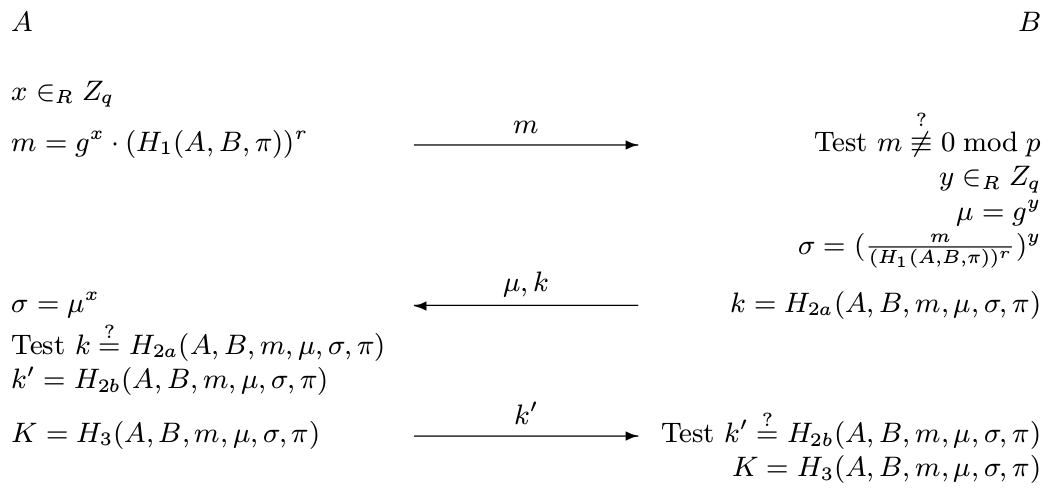
\includegraphics[scale = 0.26]{pak_protocol.png}
 \end{center}
 \end{itemize}

}

\frame{  
  \frametitle{PAK/PPK -- PPK}

   \begin{itemize}
    \item[\textbf{Setup}] Let $G = <\hspace{-.05in} g \hspace{-.05in} >$ be an order $q$ subgroup of $\mathbb{Z}_p^*$
 \item[] Let $p = rq+1$ where $r, q$ relatively prime.
 \item[] Let $\pi$ be the password and $H_1, H_3$ be random, independent hash functions.
 \item[]\pause
 \item[\textbf{PPK}]
 \item[]
 \begin{center}
 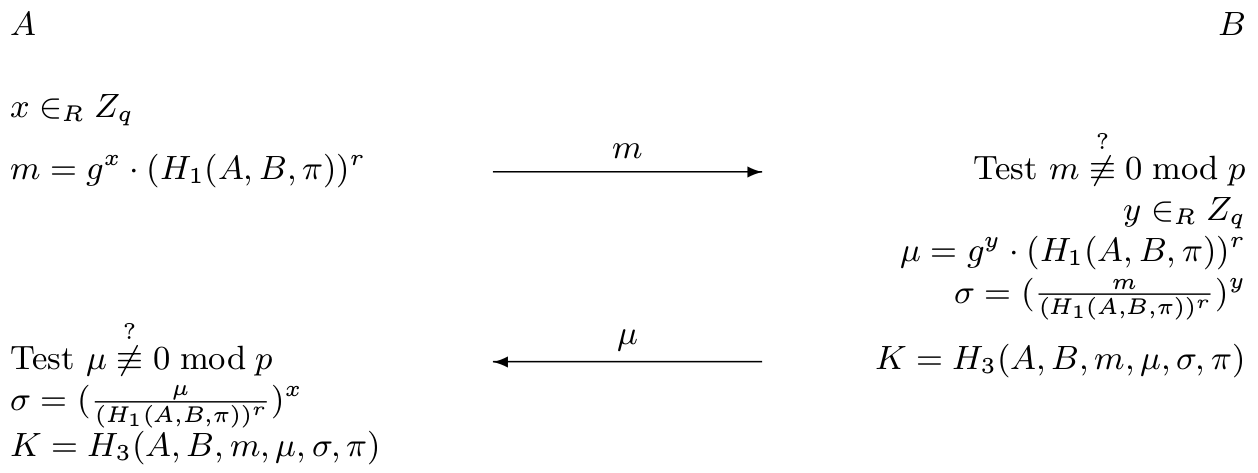
\includegraphics[scale = 0.23]{ppk_protocol.png}
 \end{center}
 \end{itemize}
 
}

\frame{  
  \frametitle{PAK/PPK}
  
  Proposes a new formal security model\\
  based on the random oracle model
  \vspace{0.4in}
  
   Satisfies all 4 desired properties \\
   (under DDH assumptions)
   \vspace{0.4in}

   Only two/three rounds of communication
   \vspace{0.4in}

   PAK has explicit key confirmation\\
   PPK has implicit key confirmation

}

\frame{  
  \frametitle{Comparisons}
  
  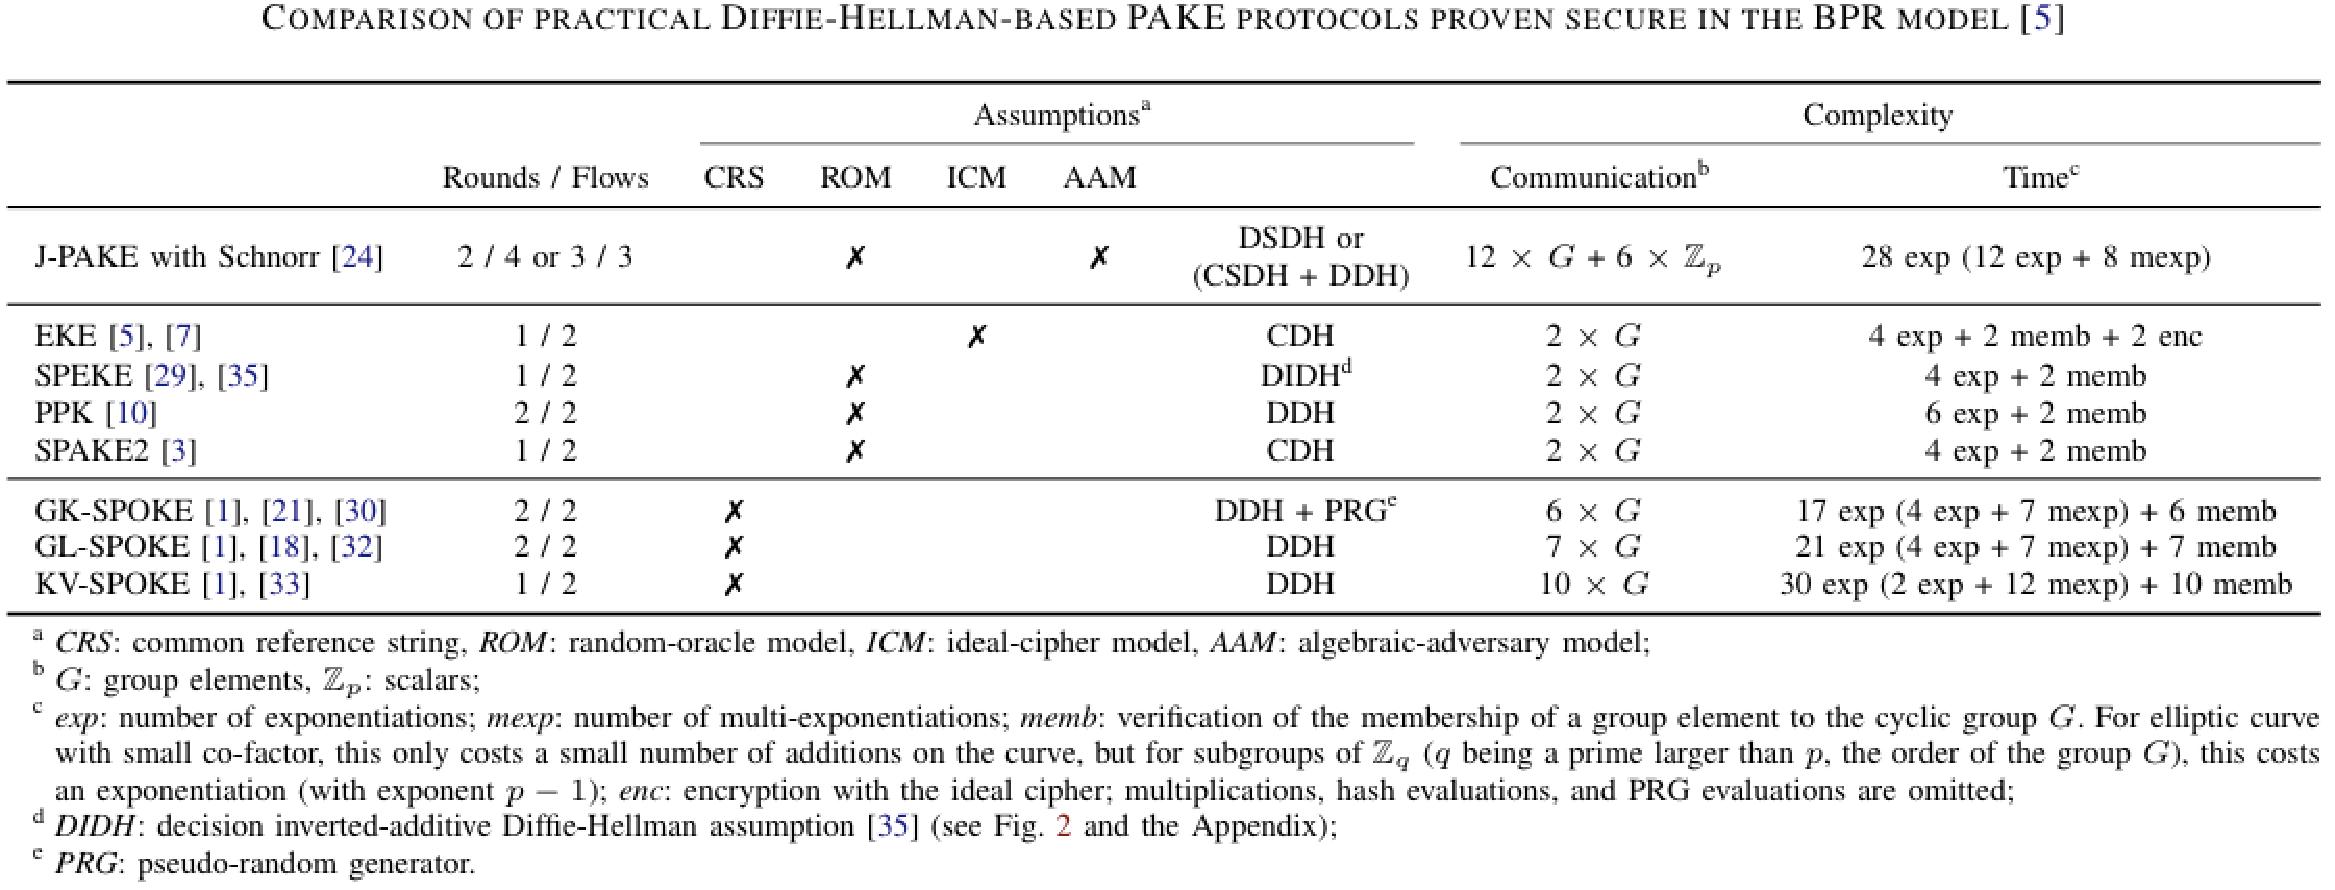
\includegraphics[width=\linewidth]{Comparisons.pdf}
  \vspace{0.2in}

  {\tiny Security of the J-PAKE Password-Authenticated Key Exchange Protocol. \\
  M. Abdalla, F. Benhamouda and P. MacKenzie, SP'2015.}
  

}

%%%%%%%%%%%%%%%%%%%%%%%%%%%%%%%%%%%
% GPAKEs
%%%%%%%%%%%%%%%%%%%%%%%%%%%%%%%%%%%

\frame{
  \frametitle{\vspace{1.1in} \begin{center} PART 2 \\ Extension to Group Setting \end{center}}
}

\frame{  
  \frametitle{The Fairy-Ring Dance}
  Group members establish the group key and the pair-wise keys simultaneously.
  \vspace{0.2in}
  
  \pause
  \textbf{For pair-wise key:}\\
  Use plain two-party PAKE protocols. (Need at least 2 rounds)
  
  \vspace{0.2in}
  
  \pause
  \textbf{For group key:}\\
  \begin{itemize}
  \item Everyone additionally choose another random $y_i \in_R \mathbb{Z}_q$ and broadcast $g^{y_i}$
  \item Everyone can calculate $g^{z_i} := g^{y_{i+1} - y_{i-1}} = g^{y_{i+1}}/g^{y_{i-1}}$
  \end{itemize}
  
  \pause
  Group key:
  \begin{align}
  \label{groupkey}
  K_i &= (g^{y_{i-1}})^{ny_i} \cdot (y^{z_iy_i})^{n-1} \cdot (y^{z_{i+1}y_{i+1}})^{n-2} \cdots (g^{z_{i_2}y_{i-2}})\\
  &= g^{y_1y_2+y_2y_3+\cdots+y_ny_1}
  \end{align}  
}

\begin{frame}{Dragonfly+}
    \begin{itemize}
        \item[\textbf{Setup}] Let $Q$ be a cyclic subgroup of $\mathbb{Z}_p^*$ with prime order $q$ with generator $g$.
            Each member maps the password to an element $\pi \in Q$.
        \item[] Every member $P_i$ chooses $r_{ij}, m_{ij} \in_R \mathbb{Z}_q^*$ for all $j \in \{1,\ldots,n\} \setminus \{i\}$
        \item[] Each member also chooses $y_i \in_R \mathbb{Z}_q$ and computes $g^{y_i} \mod p$
        
        \item<2->[\textbf{Rd 1}] Each member broadcasts $s_{ij} = r_{ij} + m_{ij} \mod q$ and $E_{ij} = \pi^{-m_{ij}} \mod p$
        \item<2->[] They also broadcast $g_{y_i} \mod p$ along with $\text{ZKP}\{y_i\}$
        \item<2->[] [All members verify the ZKP, verify $g_{z_i} \neq 1$ and check for reflection attacks]
    \end{itemize}
\end{frame}

\begin{frame}{Dragonfly+}
    \begin{itemize}
        \item[\textbf{Rd 2}] Each member computes their pairwise shared secrets: $ss_{ij} = (\pi^{s_{ji}} E_{ji})^{r_{ij}}$
        \item[] Each member broadcasts $H(ss_{ij} || E_{ij} || s_{ij} || E_{ji} || s_{ji})$
        \item[] [All members verify the pairwise hash values]
        
        \item<2->[\textbf{Rd 3}] Every member broadcasts $(g^{z_i})^{y_i}$ and $\text{ZKP}\{\tilde{y_i}\}$.
        \item<2->[] Let $K_{ij}$ be the pairwise Dragonfly key between members $i$ and $j$. Members compute
            $\kappa_{ij}^{MAC} = H(K_{ij} || "MAC"), \kappa_{ij}^{KC} = H(K_{ij} || "KC")$
        \item<2->[] Members broadcast $t_{ij}^{MAC} = HMAC(\kappa_{ij}^{MAC},  g^{y_i} || \text{ZKP}\{y_i\} || (g^{z_i})^{y_i} || \text{ZKP}\{\tilde{y_i}\})$
            and $t_{ij}^{KC} = HMAC(\kappa_{ij}^{KC}, "KC" || i || j || E_{ij} || E_{ji})$
        \item<2->[] [All members verify $\text{ZKP}\{\tilde{y_i}\}$, $t_{ji}^{MAC}$ and $t_{ij}^{KC}$ are correct]
    \end{itemize}
    \uncover<3>{
        All members share:
            \[ K = g^{y_1 \cdot y_2 + y_2 \cdot y_3 + \cdots + y_n \cdot y_1} \]
    }
\end{frame}

%%%%%%%%%%%%%%%%%%%%%%%%%%%%%%%%%%%
% Timings
%%%%%%%%%%%%%%%%%%%%%%%%%%%%%%%%%%%

\frame{
  \frametitle{\vspace{1.1in} \begin{center} PART 3 \\ Timings \end{center}}
}

\frame{  
  \frametitle{Specifications}
  \begin{itemize}
    \item All protocol benchmarks were implemented in Java 1.6 and run on a server (3GHz AMD processor, 6GB of RAM) running Ubuntu 12.04.
    \item[]
    \item[]
    \item Benchmarks measured latency, the amount of work each device would have to do in the group excluding communication.
  \end{itemize}
}

\frame{  
  \frametitle{Results}

  \begin{figure}\center 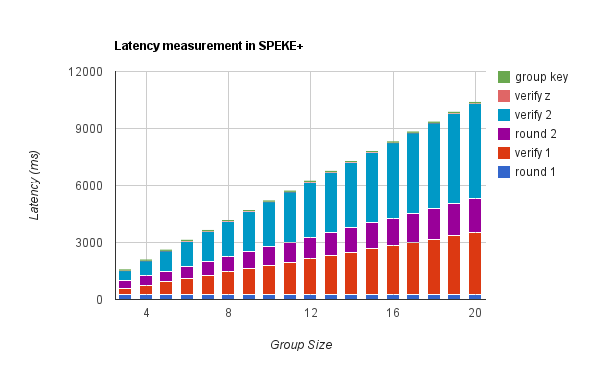
\includegraphics[scale = 0.33]{speke.png} \end{figure}

  \begin{figure}\center 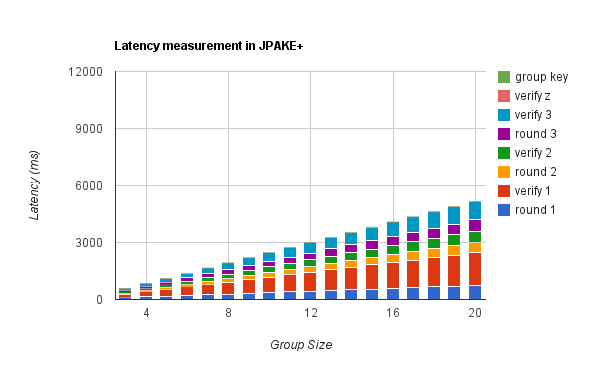
\includegraphics[scale = 0.33]{scale_jpake.png} \end{figure}
  
}

\frame{  
  \frametitle{Results}

  \begin{figure}\center 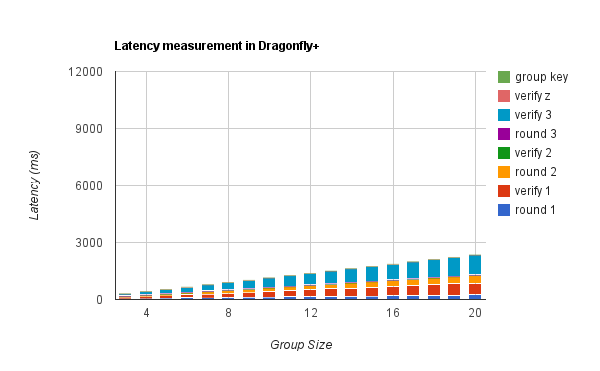
\includegraphics[scale=0.33]{scale_dragon.png}\end{figure}

  \begin{figure}\center 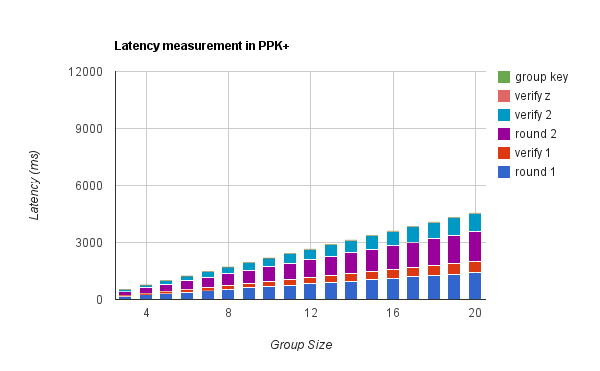
\includegraphics[scale=0.33]{scale_ppk.png}\end{figure}
  
}




%%%%%%%%%%%%%%%%%%%%%%%%%%%%%%%%%%%
% Conclusion
%%%%%%%%%%%%%%%%%%%%%%%%%%%%%%%%%%%

\frame{
  \frametitle{\vspace{1.1in} \begin{center} Conclusion \end{center}}
}

\frame{  
  \frametitle{Conclusion}
  \begin{itemize}
  \item[] It is possible to transfer PAKEs into GPAKEs while preserving round efficiency
  \item[]
  \item[] SPEKE+ is very slow
  \item[]
  \item[] J-PAKE+ is a bit slow, but proven secure (under DSDH)
  \item[]
  \item[] PPK is faster 
  \item[]
  \item[] Dragonfly is fastest, but no security proof 
  \item[] (despite IEEE 802.11-2012 standard)
  \end{itemize}
}



\frame{
  \frametitle{\vspace{1.1in} \begin{center} THANK YOU \end{center}}
}

\end{document}


